% !TEX TS-program = pdflatex
% !TEX encoding = UTF-8 Unicode
%% For double-blind review submission
\documentclass[acmsmall,screen]{acmart}\settopmatter{printfolios=true}
%% For single-blind review submission
%\documentclass[acmlarge,review]{acmart}\settopmatter{printfolios=true}
%% For final camera-ready submission
%\documentclass[acmlarge]{acmart}\settopmatter{}

%% Note: Authors migrating a paper from PACMPL format to traditional
%% SIGPLAN proceedings format should change 'acmlarge' to
%% 'sigplan,10pt'.


%% Some recommended packages.
\usepackage{booktabs}   %% For formal tables:
                        %% http://ctan.org/pkg/booktabs
\usepackage{subcaption} %% For complex figures with subfigures/subcaptions
                        %% http://ctan.org/pkg/subcaption


\makeatletter\if@ACM@journal\makeatother
%\acmDOI{10.1145/nnnnnnn.nnnnnnn}
\startPage{1}
\else\makeatother
%% Conference information (used by SIGPLAN proceedings format)
%% Supplied to authors by publisher for camera-ready submission
%\acmDOI{10.1145/nnnnnnn.nnnnnnn}
\startPage{1}
\fi


%% Copyright information
%% Supplied to authors (based on authors' rights management selection;
%% see authors.acm.org) by publisher for camera-ready submission

%% Bibliography style
\bibliographystyle{ACM-Reference-Format}
%% Citation style
%% Note: author/year citations are required for papers published as an
%% issue of PACMPL.
\citestyle{acmauthoryear}   %% For author/year citations

\usepackage{uri}
\usepackage{mathtools}
\usepackage{amsthm}
%\usepackage{amssymb}
\usepackage{semantic}
\usepackage{graphicx}
\usepackage{cases}
\usepackage{hyperref}
\usepackage{stmaryrd}
\usepackage{listings}
\usepackage{iris}
%\usepackage{lstlangcoq}
\renewcommand{\lstlistingname}{Figure}

\clubpenalty = 10000
\widowpenalty = 10000
\displaywidowpenalty = 10000

\lstset{language=C,basicstyle=\ttfamily,mathescape=true,columns=fullflexible}



\newcommand{\TODO}[1]{\textbf{\textcolor{red}{[ TODO: #1]}}}
%\newcommand{\boxdotright}{\!\mathrel\boxdot\joinrel\rightarrow\!}
\newcommand{\islock}{\boxdotright}
\newcommand{\isaex}{\!\mathrel\odot\joinrel\rightarrow\!}
\newcommand{\xisaex}[1]{\!\mathrel\odot\joinrel\xrightarrow{#1}\!}
%% \newcommand{\ifthenelse}[3]{\text{if }#1\text{ then }#2\text{ else }#3}
\newcommand{\emp}{\mathsf{emp}}

\newcommand\dboxed[1]{\dbox{\ensuremath{#1}}}
\newcommand{\master}[2]{\ensuremath{\mathrm{Master}_{#1}(#2)}}
\newcommand{\snap}[1]{\ensuremath{\mathrm{Snapshot}(#1)}}
\newcommand{\ghost}[2]{\ensuremath{\dboxed{#1}^{#2}}}
\newcommand{\ifthenelse}[3]{\text{if }#1\text{ then }#2\text{ else }#3}
\newcommand{\us}{$\mu$s}

%\newcommand{\ignore}[1]{}

\hyphenation{Comp-Cert}

\usepackage[utf8]{inputenc}
\usepackage{geometry}
\geometry{a4paper}

\usepackage{graphicx} % support the \includegraphics command and options
\usepackage{verbatim} % adds environment for commenting out blocks of text & for better verbatim
%\usepackage{amssymb}
\usepackage{url}
\usepackage{listings}

\title{Verifying a Binary Search Tree with Fine-Grained Locking}
\author{Roshan Sharma}
\author{Shengyi Wang}
\author{Lennart Beringer}
\author{William Mansky}

\date{} % Activate to display a given date or no date (if empty),
         % otherwise the current date is printed 

\begin{document}
\acmConference{Some conference}
\maketitle

\catcode`\@=11
\section{Introduction}
Modern CPU design trends have shifted towards multicore processing over the last two decades. This is because the computing power of computers has reached its limit in single-threaded execution, while the quantity of transistors per single-core CPU are increasing as described by Moore's law \cite{moore}. CPUs have multiple cores now because that is the only way to get more transistors per chip, and achieve a desirable throughput. However, doubling the quantity of cores on one chip does not immediately imply an increase in the performance by a factor of two. Programs that we aim to run in multiple cores have to be carefully designed to efficiently divide the workload into threads, and facilitate non-conflicting access to the shared data by multiple threads in parallel. These challenges is resolved by designing the concurrent data structures, algorithms that provide thread-safe access to the shared data by storing and organizing data in a standard way. Concurrent data structures are now widely employed in real-world applications like database algorithms, file systems, networking, e-commerce, etc. Designing these data structures has been considered as one of the difficult tasks in the software development fields. Despite the careful design, implementation, and thorough unit testing of these algorithms, it is very likely to expect subtle bugs and unexpected behaviors of the program. This is because threads interact with each other in complex and subtle ways such that it is almost impossible to cover every corner case while testing. Therefore, it is important to use a precise way of proving the correctness of concurrent data structures which provides a guarantee that the given algorithm correctly implements the specified concurrent data structures.

Formal verification is an active field of research that aims to prove or disprove the correctness of algorithms with respect to a certain formal specification, using mathematical techniques. Model checking and theorem proving  (also called deductive reasoning) are the two main approaches in this field. Model checking builds the mathematical model of a system as a collection of states and actions that move from one state to another. The model checker then outputs yes if the given model meets the given specifications and produces a counterexample otherwise, after a systematic and exhaustive exploration of a mathematical model. Model checking approach only works for finite models and certain infinite models that can be easily abstracted into finite sets of states. While it is a simple and automated operation, it does not scale well to large and complex systems where the search spaces are typically too large to be explored in a reasonable amount of time with a reasonable amount of space. Theorem proving, on the other hand, is a more powerful technique than model checking which can deal with an infinite state space. It works by generating a collection of mathematical proof obligations from the system and its specifications and proving these obligations using either proof assistants (such as Coq, Isabelle, PVS, HOL) or using automatic theorem provers (such as SMT solvers). Theorem proving allows us to work on more accurate representations of the system and express any properties, but most proofs have to be done manually which requires time and expertise. Since the binary search tree that we target for verification is a concurrent data structure of unbounded key-value pairs, and processes. The concurrency considerably increases the state space, and we also want to work with a model that's connected to the actual behavior of C programs, while model checking usually works on more abstract models. So, we use the theorem proving approach to formalize the proof of correctness.

In this thesis, we describe the formal verification of the correctness of concurrent binary search tree with fine-grained locking. We implement the BST algorithms in C and use the Verified Software Toolchain(VST) \cite{plfcc} to verify with respect to given specification. The concurrent separation logic (CSL) is employed to reason about behavior of the program implemented in the C programming language. Separation logic (SL) \cite{seplogic} is an extension of Hoare logic \cite{hoare}, way of reasoning about programs using a set of logical rules. SL helps to locally reason about programs that play with pointer data structures, where specifications and proofs of a program component only reflect the chunk of memory that the component uses, not the entire global state of the system. Concurrent separation logic (CSL) is a variant of the separation logic for reasoning about the concurrent programs. The version of CSL formalized in VST is rooted on the work of Hobor et al. \cite{oraclesematic}, but extended with higher-order ghost state in the style of Iris \cite{higherorderghoststate}.
\section{Background}
\label{background}
\subsection{VST and Iris}
We use the Verified Software Toolchain \cite{plfcc}  to prove the correctness of the concurrent binary search tree. VST is a Coq-based proof system that helps to prove separation logic properties of C programs with the assurance that the properties will be preserved in compiled code. First, we write programs in C programming and using CompCert’s \emph{clightgen}, the ASTs for C programs can be generated in Coq. We then state and prove specifications for them using Verifiable C. Verifiable C is a higher-order separation logic for reasoning about the functional correctness of C programs and carries a soundness proof that links high-level specifications to assembly code generated by the CompCert Verified compiler. Verifiable C supports reasoning about two separate kinds of concurrency:  Pthreads-style concurrency with locks (used by implementing blocking data structures that can be fine-grained or coarse-grained ), and concurrency using C11 atomic operations (i.e. lock-free data structures). 

\subsection{Ghost State and Global Invariants}
We can prove memory safety and race freedom properties of shared-memory concurrent programs, by tracking the transfer of ownership of shared locations between threads that would happen if we ran the program. But, this idea is insufficient to prove that concurrently running threads are successful to accomplish some task, which is also called functional correctness. For instance, we can prove the memory safety properties of the increment example in  \ref{figure1} through the transfer of ownership of shared variable $x$ between threads. But, we can not guarantee that the value of $x$ will be $2$ after all threads complete their execution, which is demonstrated in \ref{figure1} using separation logic assertion.   
\begin{figure}[htb]
\centering
$\texttt{x = 0;}$\\
$\mathit{I_{\pi}(x \mapsto v \land v \geq 0)}\hspace{30px}\pi = \pi_1\ .\ \pi_2$\\
$\begin{array}{l || l}
\mathit{I_{\pi_1}(x \mapsto v \land v \geq 0)} & \mathit{I_{\pi_2}(x \mapsto v \land v \geq 0)}\\
\texttt{acquire(l);} & \texttt{acquire(l);}\\
\mathit{x \mapsto v \land I_{\pi_1}(x \mapsto v \land v \geq 0)} & \mathit{x \mapsto v \land I_{\pi_2}(x \mapsto v \land v \geq 0)}\\
\texttt{x++;} & \texttt{x++;}\\
\mathit{x \mapsto v+1 \land I_{\pi_1}(x \mapsto v \land v \geq 0)} & \mathit{x \mapsto v+1 \land I_{\pi_2}(x \mapsto v \land v \geq 0)}\\
\texttt{release(l);} & \texttt{release(l);}\\
\mathit{I_{\pi_1}(x \mapsto v \land v \geq 0)} & \mathit{I_{\pi_2}(x \mapsto v \land v \geq 0)}\\
\end{array}$\\
$\mathit{I_{\pi}(x \mapsto v \land v \geq 0)}$
\caption{The increment example annotated with separation logic assertion}
\label{figure1}
\end{figure}
We must preserve the connection between the value of shared resources and the work performed by each thread. A common approach to achieve this is to use \emph{ghost variables}, an auxiliary state introduced later in the proof to track the local information about each thread. They do not appear in the original program. Program in \ref{figure1} can be verified by creating ghost state, which tracks the latest action performed by a thread, for each thread with initial value of $0$, and update with $1$ after each thread increment the value of \texttt{x}. In VST, we can create \emph{ghost state} for any Coq type in the form of an arbitrary \emph{partial commutative monoid} (PCM), a set with a partially defined binary operation that is as associative as it can, commutative, and has a unit, as long as we can describe what happens when two elements of that type are joined together. VST provides $\mathsf {ghost\_var}$ assertion to create a simple ghost state: $\mathsf{ghost\_var}\ \mathit{sh}\ a\ g$ asserts that $g$ is a \emph{ghost name} (\textsf{gname} in Coq) associated with the value $a$, which may be of any type. We will see different kind of ghost states used to verify binary search tree in Section \ref{correctness}.

The main idea behind the logic from Iris \cite{higherorderghoststate}, a mechnized higher-order concurrent separation logic framework, is the construction of \emph{global invariant} as \emph{ghost state}. \emph{Global Invariant} is an invariant on the global (ghost and physical) state of program. We can open any invariant but must close it again before taking any steps of execution unless those execution are atomic. Thread can use the contents of \emph{global invariant} during atomic operation if it can guarantee that no one will ever see an intermediate state in which invariant does not hold. The rules from Jung et al.\cite{higherorderghoststate} for creating and opening invariants are:

$$\inference[\textsf{inv\_alloc}]{}{\triangleright P \vdash \pvs[E] \mathsf{EX}\ i : \mathsf{iname}, \knowInv{i}{P}}$$
$$\inference[\textsf{inv\_open}]{i \in E}{\knowInv{i}{P} \vdash \pvs[E][E \setminus i] \triangleright P * (\triangleright P \wand \pvs[E \setminus i][E] \mathsf{emp})}$$

where invariants are provided in the form of assertion  $\knowInv{i}{P}$, and states that $P$ is maintained as an invariant on the global state with name $i$. The operator $\pvs[][]$ is called ``fancy update" operator,that allows to allocate, open, and close the invariants and the later $\triangleright$ operator is used for impredicativity (i.e. $\knowInv{i}{..\knowInv{i}{P}..}$).
\subsection{Atomic Specifications}
\emph{Linearizability} is one of the most popular traditional correctness condition for concurrent data structures. It is defined in terms of a set of high-level operations, such as insert and remove for a set; if a data structure is linearizable, any operation performed on it tends to happen atomically and in some order that corresponds to the real-time ordering of such operations. For instance, if operation $A$ is completed before operation $B$, then $B$ should logically follow $A$. We can prove the linearizability property of concurrent data structures using \emph{global invariants}. Suppose we have an invariant that said ``there exists a linear history of operations performed on the data structures, stored in some ghost state, and the current  state of the data structure is the one that would result from applying each of those operations in order". Then this directly implies that data structure is linearizable. We can allow a data structure operation to access the content of global invariants, treating that operation as an atomic operation if we are able prove that that operation \emph{appears to execute atomically} at some linearization point. This idea was introduced in the TaDA logic \cite{tada} in the form of \emph{atomic Hoare triples} as shown below, and called as  \emph{Logical atomicity}.    
$$\forall a.\ \langle P_l\ |\ P_p(a)\rangle\ c\ \langle Q_l\ |\ Q_p(a)\rangle$$

where $P_l$ and $Q_l$ are \emph{private} pre- and postconditions similar to ordinary Hoare triple, and $P_p$ and $Q_p$ are \emph{public} pre- and postconditions, parameterized by an abstract value $a$ of shared data structure. $P_l$ and $Q_l$ are \emph{local} to each thread 
and do not interfere with global state of a data structure, while $P_p$ and $Q_p$ are public to all threads and must satisfy following rule: $P_p$ must be true at every point from the beginning of the function until the linearization point, for some abstract value $a$, and $Q_p$ must be true at the lineariztion point, but may not still true by the end of the function. So, at the linearization point the operation atomically transitions from $P_p$ to $Q_p$.

VST has encoded an atomic Hoare triple, and provide the way that matches the notation VST uses for normal specifications. Such specification is called \emph{atomic specification}, and can be formalized in Coq as shown in  \ref{atomic_spec}.  This is how we write pre- and postcondition in VST. 
\begin{figure}[htb]
\centering
\begin{verbatim}
Program Definition insert_spec :=
DECLARE _insert
ATOMIC TYPE W OBJ a INVS Ei Eo
WITH ...
PRE [ ... ]
  PROP (...)
  LOCAL (...)
  SEP (P_l) | (P_p)
POST [ ... ]
  PROP ()
  LOCAL ()
  SEP (Q_l) | (Q_p)
\end{verbatim}
\caption{Atomic Specification in VST}
\label{atomic_spec}
\end{figure}
\texttt{W} is the \textsf{TypeTree} representing the type of arguments passed with \texttt{WITH} clause; \texttt{a} is the abstract state for the triple; \texttt{Ei} and \texttt{Eo} are the sets of invariants names inside and outside the triple. The \texttt{PROP} clause describes things that that are true independent of program state, the \texttt{LOCAL} clause describes the values contained in C local variables, and the \texttt{SEP} clause represents the \emph{separating conjunction} (*) of \emph{spatial predicates}, predicates on some part of the memory. In VST, while proving that a function implements an atomic specification, the precondition will contains an $\mathsf{atomic\_shift}$ assertion with the public pre- and postcondition, and the masks inside it. This atomic shift can be accessed through following two rules:
$$\inference[\textsf{atomic\_commit}]{\forall a, R * P_p\ a \Rrightarrow \mathsf{EX}\ y,\ Q_p\ a\ y * R'\ y}{\textsf{atomic\_shift}(P_p, E_i, E_o, Q_p, Q) * R \Rrightarrow \mathsf{EX}\ y,\ Q\ y * R'\ y}$$
$$\inference[\textsf{atomic\_rollback}]{\forall a, R * P_p\ a \Rrightarrow P_p\ a * R'}{\textsf{atomic\_shift}(P_p, E_i, E_o, Q_p, Q) * R \Rrightarrow \textsf{atomic\_shift}(P_p, E_i, E_o, Q_p, Q) * R'}$$
During commit, we must provide resources $R$ which, in combination with the public precondition $P_p$, allow us to prove the public postcondition $Q_p$. Then, we gain access to an assertion $Q$ required by the postcondition of the function, and leftover resources $R'$. During rollback, we provide resources $R$ which, in combination with the public precondition, allow us to reestablish the public precondition; we then regain the atomic shift back in the proof, as well as leftover resources $R'$. The rollback is specially used to learn some relationship between pieces of information (e.g. ghost state) stored in the public precondition, while the commit is used to prove the public postcondition from the precondition, and obtain an assertion $Q$. To complete the proof of any function's specification, we must always perform commit to obtain $Q$; we can perform any number of roolbacks before that point, but after that point we lose the atomic shift and no access to the public precondition.

\section{Safety Proofs}
\label{safety}
\begin{figure}[htp]
\begin{subfigure}[t]{\textwidth}
\begin{lstlisting}[language = C]
typedef struct tree {int key; void *value; struct tree_t *left, *right;} tree;
typedef struct tree_t {tree *t; lock_t *lock;} tree_t;
typedef struct tree_t **treebox;

void insert (treebox t, int x, void *value) {
  struct tree_t *tgt = *t;
  struct tree *p;
  void *l = tgt>lock;
  acquire(l);
  for(;;) {
    p = tgt->t;
    if (p==NULL) {
      tree_t *p1 = (struct tree_t *) surely_malloc (sizeof *tgt);
      tree_t *p2 = (struct tree_t *) surely_malloc (sizeof *tgt);
      p1 ->t = NULL;
      p2 ->t = NULL;
      lock_t *l1 = (lock_t *) surely_malloc(sizeof(lock_t));
      makelock(l1);
      p1->lock = l1;
      release2(l1);
      lock_t *l2 = (lock_t *) surely_malloc(sizeof(lock_t));
      makelock(l2);
      p2->lock = l2;
      release2(l2);
      p = (struct tree *) surely_malloc (sizeof *p);
      tgt->t = p;
      p->key=x; p->value=value; p->left=p1; p->right=p2;
      release2(l);
      return;
    } else {
      int y = p->key;
      if (x<y){
      	tgt = p->left;
        void *l_old = l;
        l = tgt->lock;
        acquire(l);
        release2(l_old);
      } else if (y<x){
        tgt = p->right;
        void *l_old = l;
        l = tgt->lock;
        acquire(l);
        release2(l_old);
      }else {
      	p->value=value;
        release2(l);
      	return;
      }
    }
  }
} 
\end{lstlisting} 
\end{subfigure}
\caption{Insert Method}
\label{insert}
\end{figure}     
\begin{figure}[htp]
\begin{subfigure}[t]{\textwidth}
 \begin{lstlisting}
void *lookup (treebox t, int x) {
  struct tree *p; void *v;
  struct tree_t *tgt;
  tgt = *t;
  void *l = tgt->lock;
  acquire(l);
  p = tgt->t;
  while (p!=NULL) {
    int y = p->key;
    if (x<y){
      tgt=p->left;
      void *l_old = l;
      l = tgt->lock;
      acquire(l);
      p=tgt->t;
      release2(l_old);
    }else if (y<x){
      tgt=p->right;
      void *l_old = l;
      l = tgt->lock;
      acquire(l);
      p=tgt->t;
      release2(l_old);
    }else {
      v = p->value;
      release2(l);
      return v;
    }
  }
  release2(l);
  return NULL;
}
\end{lstlisting}
\end{subfigure}
\caption{Lookup Method}
\label{lookup}
\end{figure}
In this section, we will focus on safety proofs of concurrent binary search tree. Here safety means thread-safe. An operation of any concurrent data-structure is thread-safe if it functions correctly during simultaneous execution by multiple threads. A thread can update the data structure if it holds a sufficiently large share of the data structure so that no other thread can possibly read it. If we want to have a data structure that can be modified by multiple threads, we must move shares between threads via locks. In VST, we can use $\mathsf{lock\_inv}$ assertion to assert that there exists a lock in memory with a given invariant: $\mathsf{lock\_inv}\ \mathsf{sh}\ p\ R$ means that the current thread owns share $\mathsf{sh}$ of a lock at location $p$ with invariant $R$. We use the term \emph{lock invariant} for $R$, which is a predicate representing the resources protected by a lock. The $\mathsf{lock\_inv}$ predicate is sufficient to prove the safety properties of the concurrent data-structure. 

%We have taken binary search tree with fine-grained locking. In hand-over-hand locking mechanism, we acquire the lock for a successor before releasing the lock for a predecessor. The code for $\texttt{insert}$ and $\texttt{lookup}$ methods of concurrent binary search tree that we are interested to verify is presented in Figure 1. 
   
\subsection{Lock invariants for hand-over-hand locking}
A node of CBST have the pointer to its children, so lock invariant of a node should have the knowledge about its children.   
Whenever we release the lock for the parent node, we have to recover all resources that the parent node accessed while acquiring the lock. By releasing the parent node's lock, we would lose the information about the lock\_inv of the node and we would not be able to release the node's lock later. To solve this problem, we use \emph{recursive} lock, one whose invariant includes a share of lock itself so that we can retain lock\_inv assertion for a node even after releasing its parent's lock. In VST, we can make such an invariant using $\mathsf{selflock}$ function along with the lemma $\mathsf{selflock\_eq}$: $\forall Q\ \mathit{sh}\ p, \mathsf{selflock}\ Q\ \mathit{sh}\ p = Q * \mathsf{lock\_inv}\ \mathit{sh}\ p\ (\mathsf{selflock}\ Q\ \mathit{sh}\ p)$. We can define $\mathsf{lock\_inv}$ predicate for \emph{recursive} lock $\mathit{lock}$ as follows: $\mathsf{lock\_inv}\ \mathit{sh1}\ p\ (\mathsf{selflock}\ P\ \mathit{sh2}\ \mathit{lock})$ where $\mathit{P}$ represents the knowledge about the children of current node, $\mathit{sh1}$ and $\mathit{sh2}$ are the two halves of the writable share.

\subsection{Specification and Verification}
We begin the verification by defining a predicate $\mathsf{nodebox\_rep}(p)$ that describes the concrete representation of the tree, where $p$ is the pointer to the root node. The $\texttt{nodebox\_rep}$ predicate ties together $\texttt{lock\_inv}$ assertion for each recursive lock as follows: 
\begin{align*}
 &\mathsf{nodebox\_rep}_{\pi}(p) \triangleq  p\mapsto\ (lock,tp)\ *\ \mathsf{lock\_inv_{\pi}}(lock, \mathsf{selflock}_{0.5}(lock,R))) \\&R  \triangleq\ \exists\ pa\ pb\ \ tp\mapsto\ (pa * pb)\ *\  \mathsf{nodebox\_rep}_{0.5}(pa)\ *\ \mathsf{nodebox\_rep}_{0.5}(pb)  \end{align*}
 
 The ownership of each node's lock is divided into two halves: one half is owned by \emph{lock\ invariant} and another half is owned by node itself. But, in case of root node, we need to split one half into multiple pieces, and share those pieces to all threads such that all of them initially have the knowledge of root node.
 
 The \emph{lock}, used in the implementation of BST operations, provides \texttt{acquire} and \texttt{release} functions, which allow threads to transfer ownership of resource invariants. Their pre- and postconditions are as follows:
$$\{!!\mathsf{readable\_share}\ \mathit{sh} \land \mathsf{lock\_inv}\ \mathit{sh}\ \ell\ R\}\ \texttt{acquire}(\ell)\ \{R * \mathsf{lock\_inv}\ \mathit{sh}\ \ell\ R\}$$
$$\{!!(\mathsf{readable\_share}\ \mathit{sh} \land \mathsf{exclusive}\ R) * R * \mathsf{lock\_inv}\ \mathit{sh}\ \ell\ R\}\ \texttt{release}(\ell)\ \{\mathsf{lock\_inv}\ \mathit{sh}\ \ell\ R\}$$


The resource invariant $R$ need to be \emph{exclusive}, i.e, it can only hold once in any given state. This allows us to know that if the current thread holds the invariants, it also hold the lock. 

    
\section{Correctness Proofs}
\label{correctness}
In the previous section, we showed that how to prove concurrent data-structure is thread safe, but not functionally correct. To prove the correctness, our threads need to be able to record the information about the actions they have performed on the shared state, instead of sealing all knowledge of the shared data structure inside the lock invariant. We can accomplish this with ghost variables, a simple form of auxiliary state. Aside from the \emph{permission} on shared resources held by each thread that we used in the safety proofs, the verification of correctness properties also involves the \emph{ghost state}. In VST, any Coq type can be used as ghost state, as long as we can describe what happens when two elements of that type are joined together. We can use own predicate in VST to represent ghost state assertion as follows: $\mathsf{own}\ g\ a\ \mathit{pp}$, where $g$ is a \emph{ghost name}, $a$ is the value associated with $g$ which can be of any type, and $\mathit{pp}$ is a separation logic predicate. 


%Linearizability is one of the most popular strong correctness condition for the most of %concurrent data-structure, which implies that every operation appears to take place atomically, %in some order, consistent with the real-time ordering of those operations. 
%In order to record the action each thread performed as a linear history, we will define global %invariants using the ghost state, which are similar to lock invariants but are not associated %with any particular memory location. Instead, a global invariant is true before and after every %step of a program, acting as a publicly accessible resource. A program instruction can use the %contents of global invariant if it can guarantee that no one will ever see an intermediate state %in which the invariant does not hold. 

\subsection{Fine-grained locking and atomicity}
\label{atomicity}

To prove that an operation on a data structure satisfies a logically atomic specification, we must show that there are no visible intermediate states of the operation, i.e., that other threads see the data structure as unchanged until the linearization point at which the operation takes effect. This is often implemented with either a lock-free series of atomic memory accesses, in which case all but the last access must make changes that are considered ``invisible'', or a coarse-grained lock, in which case any changes may be made and no other thread can access the data structure until the operation is complete. Fine-grained locking presents an interesting middle ground between these two approaches: other threads may continue to access the data structure as long as they do not require a section that is currently locked, and the visible changes may be implemented with multiple non-atomic operations in the locked section.

In an Iris-style separation logic, the lock-free approach means that each atomic operation gets access to the state of the data structure stored in an atomic shift, and must either maintain its previous state or (at the linearization point) move to a new one; in the coarse-grained approach we can store the state of the data structure in a lock invariant, and the function has access to all of it throughout the critical section. With fine-grained locking, neither of these approaches quite applies as-is: there are no atomic operations by which we access the state of the data structure, but neither is there a lock whose invariant controls access to the entire structure. However, we can take a modified form of the lock-free approach, where we treat each critical section as an atomic operation that can access the atomic shift. Typically, we will perform a sequence of non-atomic operations in the body of the critical section without access to the global state of the data structure, and then (before exiting the critical section) access the atomic shift and show that we have either maintained the original state or satisfied the postcondition of the operation. In this section, we describe a general approach to associating fine-grained locks with pieces of the abstract state of a data structure, allowing them to interact with atomic shifts and be used to prove atomic specifications. (Note that this approach is not novel to us; it is adapted from something Ralf Jung worked on. We need to be more clear about the relationship.)
 We use the following rules to associate fine-grained locks with abstract state of a data structure:
\begin{align*}
    \textsf{sync\_inv}(g,sh,R) \triangleq  \exists\ a,\ R\ g\ a\ *\ \textsf{my\_half}(g,sh,a)   \end{align*}
$$\inference[\textsf{sync\_commit}]{\forall a, R * P_p\ a \Rrightarrow \exists x_1.\ \mathsf{public\_half}(g, x_1) * \exists x_0'\ x_1'.\ (x_0, x_1) \leadsto (x_0', x_1') \land \\(\mathsf{my\_half}(g, \mathit{sh}, x_0') * \mathsf{public\_half}(g, x_1') \Rrightarrow \exists y.\ Q_p\ a\ y * R'\ y)}{\textsf{atomic\_shift}(P_p, E_i, E_o, Q_p, Q) *  \textsf{sync\_inv}(g,sh,R) \Rrightarrow \mathsf{EX}\ y,\ Q\ y * R'\ y}$$
$$\inference[\textsf{sync\_rollback}]{\forall a, R * P_p\ a \Rrightarrow \exists x_1.\ \mathsf{public\_half}(g, x_1) * (\mathsf{public\_half}(g, x_1) \Rrightarrow P_p\ a * R')}{\begin{array}{c}\textsf{atomic\_shift}(P_p, E_i, E_o, Q_p, Q) * \textsf{sync\_inv}(g,sh,R)  \Rrightarrow \\\textsf{atomic\_shift}(P_p, E_i, E_o, Q_p, Q) * \textsf{sync\_inv}(g,sh,R')\end{array}}$$

The $\mathsf{sync\_inv}$ predicate associates the contribution part of ghost state $a$ for a node with ghost name $g$, along with the other concrete information about a node parameterized on $a$. In the atomic specification, we protect the $\mathsf{sync\_inv}$ using lock inside lock invariant. So, once we acquire the lock, we get access to $\mathsf{sync\_inv}$. The $\mathsf{sync\_commit}$ and $\mathsf{sync\_rollback}$, specialized with ghost state with \emph{reference pattern} ($\mathsf{my\_half}$ and $\mathsf{public\_half}$), are the versions of $\mathsf{atomic\_commit}$ and $\mathsf{atomic\_rollback}$ described in Section \ref{background}. In a commit, we must provide $\mathsf{sync\_inv}$ with resources $R$ that, in combination with the public precondition, allow us to prove the public postcondition; we then gain access to an assertion Q required by the postcondition of the function, and leftover resources $R'$. The state of the node $g$ in public precondition (described by an assertion $\mathsf{public\_half}$) must be joinable with the state described by an assertion $\mathsf{sync\_inv}$. In a rollback, we provide $\mathsf{sync\_inv}$ with resources $R$ that, in combination with the public precondition, allow us to reestablish the public precondition; we then regain the atomic shift back in the proof, as well as $\mathsf{sync\_inv}$ with the leftover resources $R$. We must use these rules before releasing the node's lock (we lose the $\mathsf{sync\_inv}$ after releasing the lock).  

technical material: definition of sync\_inv, sync\_commit and sync\_rollback
\subsection{Specification of the algorithm}
In addition to program state, the verification of concurrent program involves two aspects which do not appear in actual C program: the \emph{shares} on shared resources and \emph{ghost state} described in Section \ref{safety}. We need to extend our specification in Section\ref{safety} with \emph{ghost state} to prove the functional correctness.  
\subsubsection{Ghost States and Range}
 The main challenge in proving the properties of concurrent data structure is to abstract the data structure in a way that helps to reason about it in the concurrent setting. Krishna et al. \cite{krishna2017flow} mention in their paper that we can abstract binary search tree using appropriate bounds in each node: we can use the product of \emph{lower-bound} and \emph{upper-bound} on each node of binary tree by propagating from each node to its child the appropriate bounds on the values presents in the sub-tree. The \emph{lower-bound} and \emph{upper-bound} help us to prove that we perform the operation in the right node: for instance, if we $\mathsf{insert}$ a key in the tree, then key should be inside those two bounds. We use the term \emph{range} to represent the product of lower- and upper-bound. \ref{range_bst} shows an example of BST with each node labeled with appropriate bound propagated all the way from \emph{root} to empty \emph{leaf} nodes. 
\begin{figure}[htb]
\centering
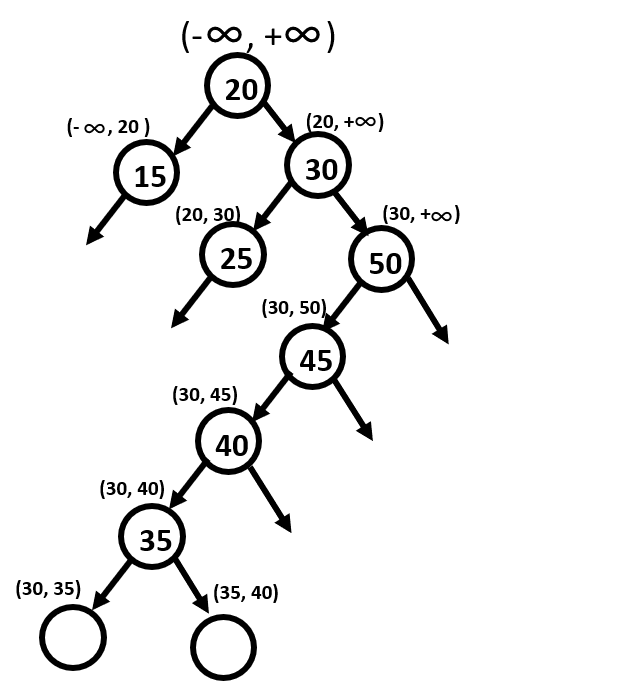
\includegraphics[width=70mm,scale=0.5]{FIG/range_prop.png}
\caption{An example of BST with each node labeled with \emph{range}; lower and upper bound for a key}
\label{range_bst}
\end{figure}
The range for root node is always $(-\infty,+\infty)$ and then, we can calculate the range for all nodes in the tree by enforcing each node to propagates appropriate bounds. For the left child, range will be lower-bound for the node (lower-bound) and the key in the node (upper-bound), while for the right child range will be a key in the node (lower-bound) and upper-bound for the node (upper-bound). This properties in each node help us to prove that the thread have changed the state of data-structure to the valid state. For instance, we can confirm that a key has been inserted in the right place if a key is inside the range of the node. Suppose we want to insert a key $38$ in \ref{range_bst}, then we will locate \emph{right} child of $35$ as the right place for $38$. During insertion, we can confirm that the node is indeed right place for $38$ by checking that $38$ is in the range (35,40). We introduce the $range$ in our proof using the ghost variables. This $ranges$ along with other information about the node represent the abstract state of the data-structure. We have used two kind of ghost state in our proof: \emph{per-node} ghost state and \emph{over-all} ghost state.\\
\textbf{Per-node Ghost State}: The per-node ghost state is the product of the range and other information about node (key, value, and ghost name for its child nodes), created for each node. In VST, to use any Coq type as a ghost state, we need to create an instance of \texttt{Ghost} typeclass, \emph{separation algebra} with associated \texttt{join} relation, with an additional \texttt{valid} predicate marking those elements of the algrebra that can be used in ghost assertions. \texttt{Ghost} typeclass is related to the PCMs described in \ref{chapter2}. For instance, ghost instance for range can be created as follows:
\begin{verbatim}
 Program Instance range_ghost : Ghost :=
  { G := (number*number); valid g := True; Join_G a b c := c =  merge_range a b }.
\end{verbatim}
Where \texttt{number} $\in (-\infty,+\infty)$ and $\texttt{merge\_range}$ is a function that merges two ranges into one. We extend this range information with the other information about the node: key, value and $\texttt{gname}$ for its child. We define our total ghost state as follows:
\begin{verbatim}
Definition ghost_info : Type := (key * val * gname * gname)%type.
Instance node_ghost : Ghost := prod_PCM range_ghost (exclusive_PCM (option ghost_info)).
\end{verbatim}
The \texttt{exclusive\_PCM} is an exlusive algebra, which means that \texttt{Some} only joins with \texttt{None}, not with another \texttt{Some} (even the same one). Now, we use ghost assertion to represent this instance. This ghost state follow \emph{reference} pattern: each thread holds partial information describing its contribution to the shared state, and the shared resources hold a "reference" copy that records all of the contributions. VST provides \texttt{my\_half} and \texttt{public\_half} assertions for this: contribution element $\mathsf{my\_half}\ \mathit{g}\ \mathit{sh}\ a$ and reference element $\mathsf{public\_half}\ \mathit{g}\ r$. To join two elements, we combine the shares and values of the contributions, and require that the elements contain at most one reference between them to ensure the uniqueness of the reference value. When \texttt{my\_half} element has the full share, it is guaranteed to be equal to the reference element. In our case, \texttt{my\_half} assertion will be local to a thread (that means it will stay in private pre- and postcondition of atomic specification), and  \texttt{public\_half} will be shared with all threads (that means public pre-and postcondition).

\textbf{Over-all Ghost State}: We have constructed the per-node ghost state for each node, using unique ghost variable for each node. But if we are given a ghost variable (\emph{gname}) to access the resources in the node labeled with that variable, we do not any clue about whether or not that variable exists in the tree. So, we need another kind of ghost state, which represents the a set of all per-node ghost variable. Again We can use ``reference" pattern to define this ghost state:
\begin{verbatim}
Definition ghost_ref g r1 := ghost_reference(P := set_PCM) r1 g.
Definition in_tree g g1 := EX sh: share, ghost_part(P :=set_PCM) sh (Ensembles.Singleton g1) g.
\end{verbatim}
We use $\mathsf{ghost\_ref}$ and $\mathsf{in\_tree}$ in the public and private part of the atomic specification respectively. The global invariant, which we introduced in our atomic specification as $\mathsf{tree\_rep}$ predicate above, ties together $\texttt{public\_half}$ and $\texttt{ghost\_ref}$ as follows:
\begin{align*}\mathsf{tree\_rep}(T,g) \triangleq [\ \forall n. \mathsf{public\_half\textsubscript{gn}} \ (\mathit{range}_n* \mathit{ghost\_info}_n)\ ] *\ \mathsf{ghost\_ref}\ g\ \{ gn\  \} \end{align*}
 Later while writing atomic specification, we will use $\mathsf{ghost\_ref}$ and $\mathsf{in\_tree}$ in the public and private part respectively. Once we open \emph{global invariant}, we get access to $\mathsf{ghost\_ref}$ which will be used with $\mathsf{in\_tree}$ to establish the fact that node actually exists in the tree. We proved the following lemma for this:
$$
Lemma\ \mathbf{\ node\_exist\_in\_tree : }\ \forall\ g\ s\ g\_in,\  \mathbf{in\_tree}\ g\ g\_in  * \mathbf{ghost\_ref}\ g\ s\ \Rightarrow\ g\_in\ \in s .
$$
\subsubsection{Combining all pieces in atomic specification}
We combine pieces of information discussed above, \emph{recursive lock invariant} from \ref{safety} and \emph{ghost states}, to write the atomic specification. The private pre- and postcondition of the atomic specification is given by defining the predicate $\mathsf{nodebox\_rep}(p,g,g\_root)$ that describes the concrete state of the BST along with the contribution part of the both kind of ghost states explained above.The root node $p$ is represented by ghost name $g\_root$ and over-all ghost state is represented by ghost name $g$. The $\mathsf{nodebox\_rep}$ predicate ties together $\mathsf{my\_half}$ part of per-node ghost state and $\mathsf{in\_tree}$ of over-all ghost state inside the $\mathsf{lock\_inv}$ assertion of each node's lock as follows:
\begin{align*}
    &\mathsf{nodebox\_rep}_{\pi}(p,g,g\_root) \triangleq  p\mapsto\ (lock,tp)\ *\ \mathsf{lock\_inv_{\pi}}(lock, \mathsf{selflock}_{0.5}(lock,R))) \\&R  \triangleq\ \ghost{\mathsf{my\_half}(range,info)}{g\_root}\ *\ \ghost{\mathsf{in\_tree}\ (g\_root)}{g}\ *\ \exists\ pa\ pb\ ga\ gb,\ tp\mapsto\ (pa * pb)\ *\  \mathsf{nodebox\_rep}_{0.5}(pa,g,ga) \\& *\ \mathsf{nodebox\_rep}_{0.5}(pb,g,gb))\end{align*}
    
The $\mathsf{nodebox\_rep}$ is a predicate describing the local information about the node almost similar to the predicate we defined for the safety proof in Section \ref{safety}. In this case, the lock invariant of recursive lock have, along with the information about the children node,$\mathsf{my\_half}$ predicate which holds the partial information describing the current thread's contribution to the shared state.

The public pre- and postcondition of the atomic specification is given by defining the predicate $\mathsf{tree\_rep}(T,g)$ that describes the abstract state of the binear search tree $T$  in terms of collection of ghost states each describing the information about separate node in the tree.. The $\mathsf{tree\_rep}$ predicate ties together $\mathsf{public\_half}$ part of per-node ghost states and $\mathsf{ghost\_ref}$ of over-all ghost state as follows: \begin{align*}&\mathsf{ghost\_tree\_rep}(tg,range, g, g\_current) \triangleq\ \exists\ k, v, ga, gb\ \in tg,\ghost{\mathsf{public\_half}\ (range, Some(k,v,ga,gb))}{g\_current}\\& *\ \mathsf{ghost\_tree\_rep}(left(tg),(left(range),k),g,ga)\ *\ \mathsf{ghost\_tree\_rep}(right(tg),(k, right(range)),g,gb) \end{align*}
\begin{align*}\mathsf{tree\_rep}(T,g,g\_root) \triangleq \ \exists\ (tg:ghost\_tree),\ &\mathsf{pure\_tree}(tg)\ =\ T\ \land\ \mathsf{ghost\_tree\_rep}(tg,(-\infty, +\infty),g,g\_root)&\\ *\ \ghost{\mathsf{ghost\_ref}\ (\mathsf{find\_ghost\_set}(tg))}{g}\end{align*}
Where $tg$ is called \emph{ghost tree}, which can be existentially quantified, extend the node in pure tree $T$ with actual pointer and ghost names for child nodes. 

The atomic specification for any binary search tree's operation \texttt{op} can be written as follows:
\begin{align*}\forall t.\ \langle \mathsf{nodebox\_rep}(p,g,g_{\mathit{root}})\ |\ \mathsf{tree\_rep}(t,g)\rangle\ \texttt{op}(p)\ \langle \mathsf{nodebox\_rep}(p,g,g_{\mathit{root}})\ |\ \mathsf{tree\_rep}(t', g)\rangle
\end{align*}

Where $t$ and $t'$ are the abstract state of a tree before and after the function's execution.

\subsection{Insert and Lookup}

\subsubsection{insert}
The C outline-code for the insert method of binary search tree is shown in \ref{insert}. A node has a lock, key, value, and pointers to the left and right child. Each leaf node in tree are empty node with lock. Whenever a thread try to insert key-value pair in the tree, it first spans the tree to find the right position for new key using hand-over-hand locking mechanism; acquire the lock for child before releasing the lock for node. After locating right leaf node to insert new key-value, thread creates two new empty leaf nodes, insert key-value in the current node, and link the newly created leaf nodes to the current node. If the key already exist in the tree, then thread simply swaps the old value associated with node with the new value keeping the child pointers as it is.

The atomic specification for insert method can be written as follows:
$$\forall t.\ \langle \mathsf{nodebox\_rep}(p,g,g\_root)\ |\ \mathsf{tree\_rep}(t,g)\rangle $$ 
$$\texttt{insert}(p,k,v)$$
$$\langle \mathsf{nodebox\_rep}(p,g,g\_root)\ |\ \mathsf{tree\_rep}(t[k\mapsto v],g)\rangle $$
We are not guaranteed that the state of  a tree at the end of the insertion will be $t[k\mapsto v]$ where $t$ is the tree state when insert is called; rather, we know that p always holds some tree during the function's execution, and at some point the function will take that tree $t$, add $[k\mapsto v]$, and then eventually return, while in the meantime another thread may have modified the state of tree from $t[k\mapsto v]$ to any other arbitrary state that the current thread do not know.

Since we have given the specification that is strong enough to specify both the safety and the functional correctness properties of insert method, we can now verify that body of the function satisfies the atomic specification given above using various VST and Iris (encoded in VST) tactics. Once we have outermost specification for a function, the another creative part in verification is finding the right loop-invariant. We defines the loop invariant for the insert function as follows: 
\begin{align*} &\mathsf{insert\_inv}(b, x, g, g\_root) \triangleq\ \exists\ \mathit{lock},\mathit{g\_current},\mathit{np},\mathit{range},\mathit{info},\ (x\in \mathit{range})\ \land \ \ghost{\mathsf{my\_half}(\mathit{range},\mathit{info})}{g\_current}\ *\ R\ \mathit{np}\\& * \mathsf{lock\_inv}(\mathit{lock},\mathit{lsh2},R')\ *\ \mathsf{nodebox\_rep}(b,g,\mathit{g\_root})\ *\ \mathsf{atomic\_shift} (P_p,E_i,E_o,Q_p,Q) \end{align*}   

Where $\mathsf{P_p}$ and $\mathsf{Q_p}$ are $\mathsf{tree\_rep}(t,g)$ and $\mathsf{tree\_rep}(t[k\mapsto v],g)$ respectively. The resources $\mathsf{R}$, parameterized by a node pointer $np$, describes the concrete information about a node. Also, $x$ is the key to be inserted that must be in the bound $\mathsf{range}$.  This loop invariant has some existential variables which characterized the state of each iteration of loop in the C code.

Figure \ref{insertproof} shows the $\texttt{insert}$ function annotated with separation logic specification. The proof starts with $\mathsf{nodebox\_rep}$ and $\mathsf{atomic\_shift}$ as the precondition. After acquiring the lock for the root node, the thread accesses the information inside the lock invariant of the root node. In order to prove $\mathsf{while}$ loop, we show that the precondition satisfies the $\mathsf{insert\_inv}$, then prove that the loop body preserves the loop invariant ( cases inside $\mathsf{else if}$ clauses at line 15 and 17 in \ref{insert}).   Once we locate the empty node for inserting new key-value pair (i.e inside the first $\mathsf{if}$ clause), we open the global invariant encoded in the $\mathsf{atomic\_shift}$, create the ghost names $\texttt{g1}$ and $\texttt{g2}$ for two new empty child nodes of current node, and prove that insertion satisfy the public postcondition $\mathsf{tree\_rep}(t[k\mapsto v],g)$ with the help of $\mathsf{sync\_commit}$ rule described in section \ref{atomicity}. This is the \emph{linearization point} of the $\mathsf{insert}$ operation and must be done at any point in the proof, but before releasing the current node's lock (i.e in critical section). In order to prove the public postcondition $\mathsf{tree\_rep}(t[k\mapsto v],g)$, we need to first locate the current node in $\mathsf{tree\_rep}(t,g)$ using ghost name $g\_current$, and then perform necessary modification such that the final state of the global invariant satisfies $\mathsf{tree\_rep}(t[k\mapsto v],g)$. We create and prove separate lemma for this, called $\emph{extract}$ lemma which is depicted in the \ref{extract_insert}.  

With the help of $\mathsf{in\_tree}$ assertion, we locate a leaf node denoted by ghost name $g\_current$ in the global state $\mathsf{tree\_rep}(t,g)$. Then we prove the \emph{extract} lemma, which says that the state of tree after adding new key-value pair (k,v) will be $\mathsf{tree\_rep}(t[k\mapsto v],g)$, by applying induction in $t$. 

Another important step in the $\mathsf{insert}$ proof is the case when we find that the key to be inserted already exists in the tree (i.e. the last $\texttt{else}$ clause in C code). The modification of the global state of the tree t is shown in \ref{extract_insert2}. In that case, the old value $v'$ associated with key is overridden by new value $v$ keeping a key $40$ and child pointers as as they are. This is also the \emph{linearization point} of the $\mathsf{insert}$ operation. We augment the same $\emph{extract}$ lemma with the clause that states the scenario in \ref{extract_insert2}, and prove the lemma in the same induction over the tree $t$.

In the rest two cases, the $\texttt{insert}$ method compares the key
of the current node with the key $\texttt{x}$ and goes down into the
corresponding left or right branch. We need to show that the range in
the ghost state shrinks correctly. To achieve this goal we open the
global invariant encoded in the $\mathsf{atomic\_shift}$ to retrieve
the necessary information. But this time these operations maintain the
original state. For the left branch case, we accomplish the proof by
the following lemma:
\begin{verbatim}
Lemma in_tree_left_range:
  forall (B: Type) (b: tree -> B -> mpred) (Q : B → mpred) (x x0: Z) (g g_root : gname)
    (inv_names : invG) (v: val) (g_in ga gb: gname) (r a: node_info),
    check_key_exist' x r.1 = true -> r.2 = Some (Some (x0, v, ga, gb)) -> x < x0 ->
    atomic_shift (λ BST : tree, !! sorted_tree BST && tree_rep2 g g_root BST) ∅ ⊤
                 b Q * my_half g_in gsh1 r * in_tree g g_in * my_half ga gsh1 a
    |-- atomic_shift (λ BST : tree, !! sorted_tree BST && tree_rep2 g g_root BST) ∅ ⊤
    b Q * my_half g_in gsh1 r *
    (EX ba, !! (less_than_equal ba r.1.1 = true /\
                range_inclusion a.1 (ba, Finite_Integer x0) = true) &&
            (in_tree g g_in * my_half ga gsh1 (ba, Finite_Integer x0, a.2))).  
\end{verbatim}
The lemma for the right branch case is similar. Both use the
$\texttt{sync\_rollback}$ lemma described in section \ref{atomicity}.
  
\begin{figure}[htb]
\centering
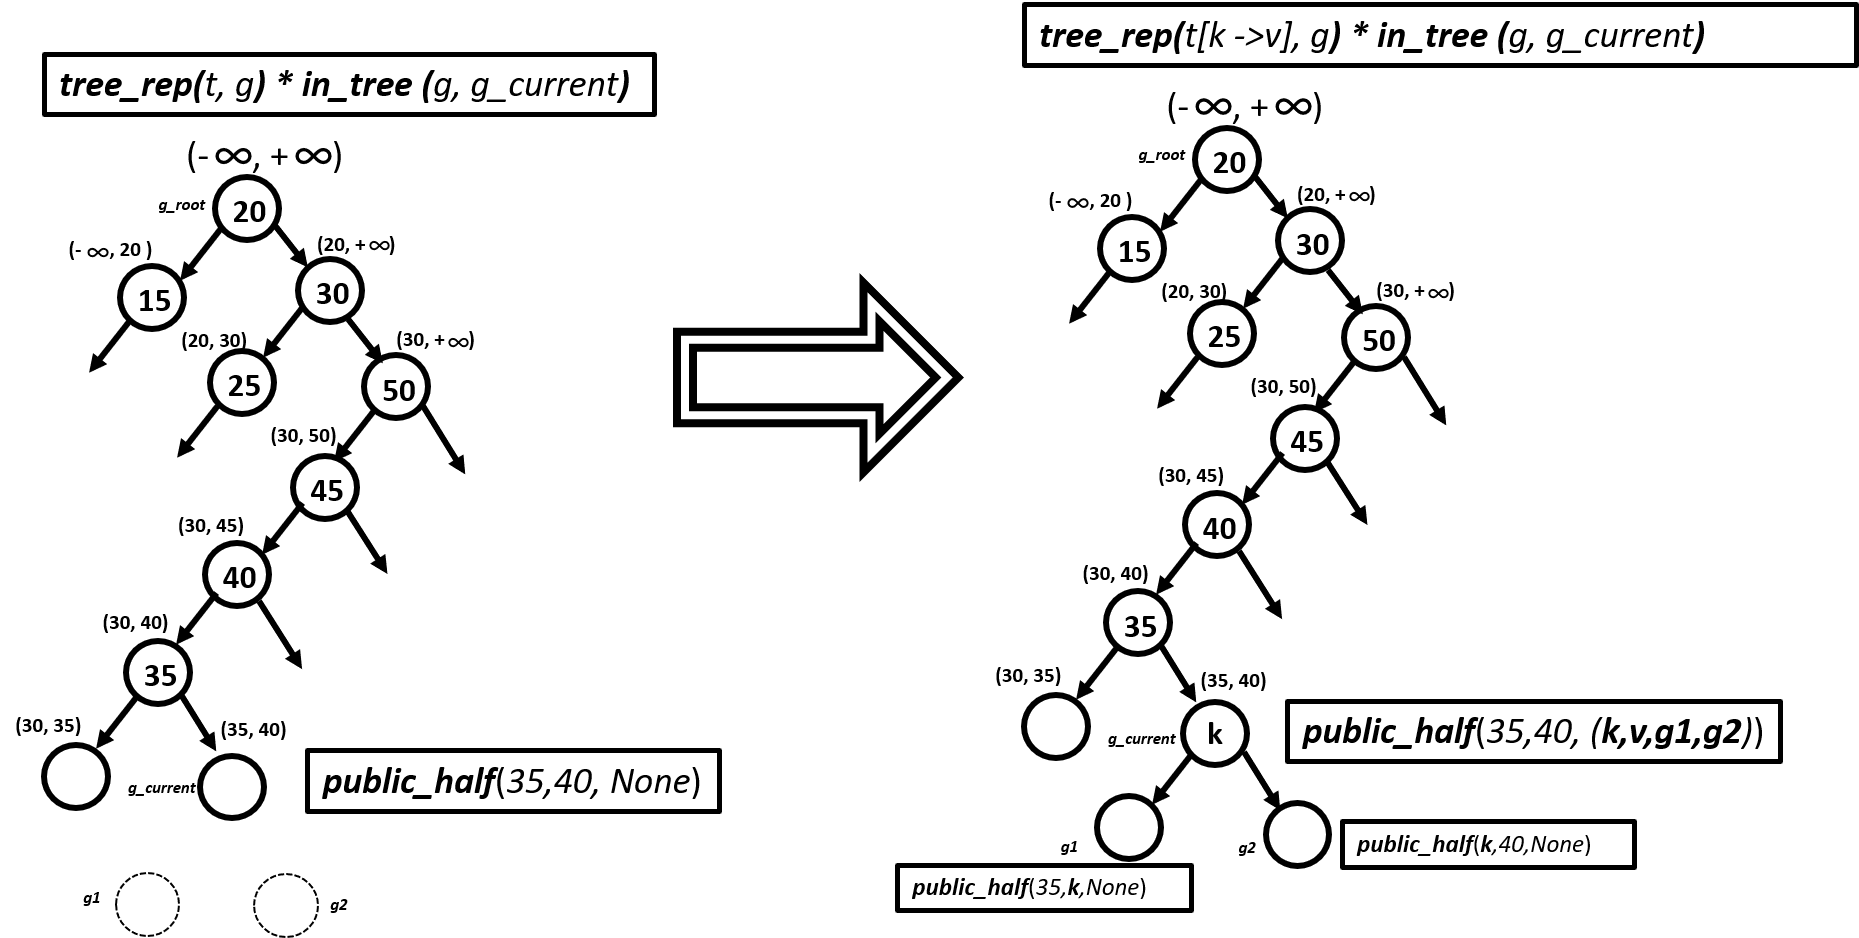
\includegraphics[width=150mm,scale=0.5]{FIG/extract_insert.png}
\caption{A visual depiction of the change in global state of BST during $\mathsf{insert(k,v)}$ operation }
\label{extract_insert}
\end{figure}
\begin{figure}[htb]
\centering
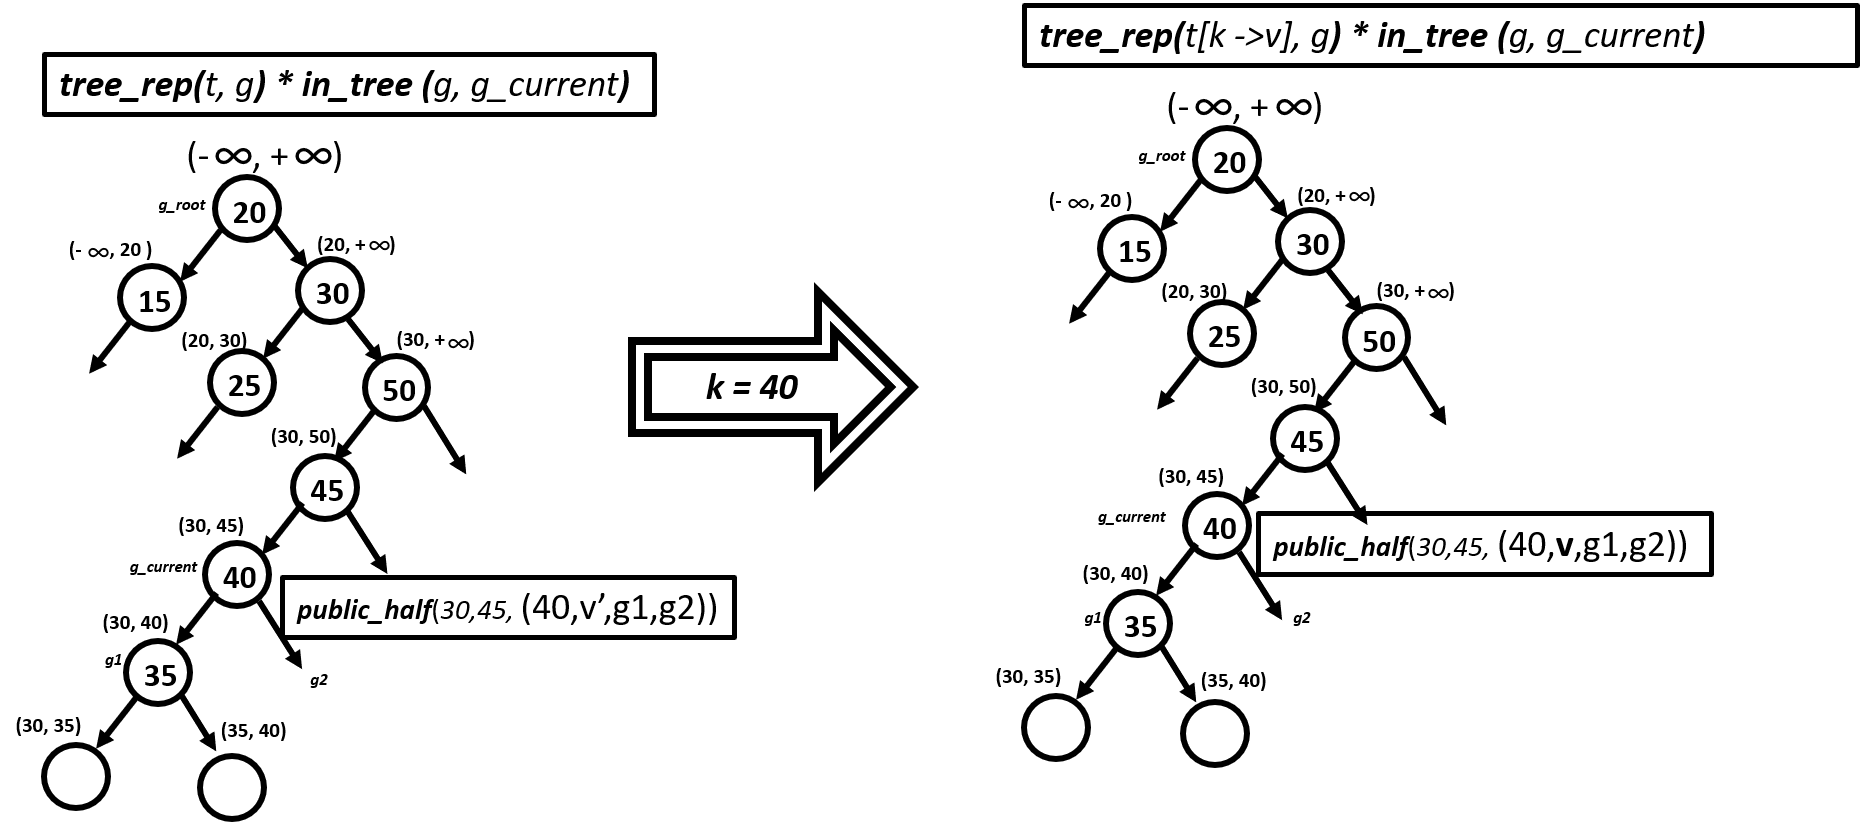
\includegraphics[width=150mm,scale=0.5]{FIG/extract_insert_2.png}
\caption{A visual depiction of the change in global state of BST during $\mathsf{insert(k,v)}$ operation, where key $k$ already exists in the tree $t$ }
\label{extract_insert2}
\end{figure}
\begin{figure}[htp]
\begin{subfigure}[t]{1\textwidth}
 $$\left\{\begin{array}{l} \mathsf{nodebox\_rep}(b,g\_root)\ *\ \mathsf{atomic\_shift}(P_p,E_i,E_o,Q_p,Q)\end{array}\right\}$$
 \vspace*{-20pt}
\begin{lstlisting}[language = C,numbers = none]
insert(treebox t, int x, void *value)
  tree_t *tgt = *t;
  acquire(tgt->lock)
 \end{lstlisting}  
 $$\left\{\begin{array}{l} \ghost{\mathsf{my\_half}((-\infty,+\infty),info)}{g\_root}\ *\ R\ b\ *\ \mathsf{lock\_inv}(lock,lsh2,R')\ *\ \\
 \mathsf{nodebox\_rep}(b,g\_root)\ *\ \mathsf{atomic\_shift}(P_p,E_i,E_o,Q_p,Q)\end{array}\right\} \Rrightarrow \left\{\begin{array}{l} insert\_inv \end{array}\right\}$$ 
  \begin{lstlisting}[language = C,numbers = none]
  for(;;) {
       \end{lstlisting}   
   $$\left\{\begin{array}{l} insert\_inv \end{array}\right\} \triangleq \left\{\begin{array}{l}(x\in range)\land \ghost{\mathsf{my\_half}(range,info)}{g\_current}*\ R\ np\ \\*\mathsf{lock\_inv}(lock,lsh2,R')\ *\ \mathsf{nodebox\_rep}(b,g\_root)\ *\ \mathsf{atomic\_shift}(P_p,E_i,E_o,Q_p,Q)\end{array}\right\}$$
      \begin{lstlisting}[language = C,numbers = none]
    p = tgt->t;
    if (p==NULL)
      tree_t *p1, *p2 = malloc();
      p = malloc(); tgt->t = p;
      p->key=x; p->value=value; p->left=p1; p->right=p2;
           \end{lstlisting} 
  $$\left\{\begin{array}{l} \ghost{\mathsf{own}\ (a1)}{g1}\ *\ \ghost{\mathsf{own}\ (a2)}{g2}\ *\ \ghost{\mathsf{my\_half}(range,None)}{g\_current}*\ R\ np\ \\*\mathsf{lock\_inv}(lock,lsh2,R')\ *\ \mathsf{nodebox\_rep}(b,g\_root)\ *\ \mathsf{atomic\_shift}(P_p,E_i,E_o,Q_p,Q)\end{array}\right\} \Rrightarrow{\textbf{sync\_commit}}$$
$$\left\{\begin{array}{l} \ghost{\mathsf{my\_half}(range,None)}{g\_current}*\ R\ np\ *\mathsf{lock\_inv}(lock,lsh2,R')\ *\ \mathsf{nodebox\_rep}(b,g\_root)\ *\ Q\end{array}\right\}$$
 \vspace*{-10pt}
        \begin{lstlisting}[language = C,numbers = none]
      release2(l);
         \end{lstlisting}
       $$\left\{\begin{array}{l} \mathsf{nodebox\_rep}(b,g\_root)\ *\ Q\end{array}\right\}$$
        \vspace*{-10pt}
         \begin{lstlisting}[language = C,numbers = none]
      return;
     else 
        ....
       else 
      	p->value=value;
      	\end{lstlisting} 
$$\left\{\begin{array}{l} \ghost{\mathsf{my\_half}(range,None)}{g\_current}*\ R\ np\ *
\mathsf{lock\_inv}(lock,lsh2,R')\ *\ \\\mathsf{nodebox\_rep}(b,g\_root)\ *\ \mathsf{atomic\_shift}(P_p,E_i,E_o,Q_p,Q)\end{array}\right\} \Rrightarrow{\textbf{sync\_commit}}$$
$$\left\{\begin{array}{l} \ghost{\mathsf{my\_half}(range,None)}{g\_current}*\ R\ np\ *\mathsf{lock\_inv}(lock,lsh2,R')\ *\ \mathsf{nodebox\_rep}(b,g\_root)\ *\ Q\end{array}\right\}$$
         \vspace*{-10pt}
      	\begin{lstlisting}[language = C, numbers = none]
        release2(l);
        \end{lstlisting}
        $$\left\{\begin{array}{l}  \mathsf{nodebox\_rep}(b,g\_root)\ *\ Q\end{array}\right\}$$
         \vspace*{-10pt}
        \begin{lstlisting}[language = C, numbers = none] 
      	return;
\end{lstlisting}
\end{subfigure}
\caption{The $\texttt{insert}$ function annotated with separation logic specification}
\label{insertproof}
\end{figure} 


\subsubsection{lookup}

The code for the $\mathsf{lookup}$ method is shown in \ref{lookup}. It takes the location of the root pointer and a key as the arguments. A thread spans the tree to find a given key using hand-over-hand locking mechanism. Once a thread finds the key in the tree, it gets the value associated with that key, release the current node's lock, and return the value. 

The atomic specification for $\mathsf{lookup}$ method can be written as follows:
\begin{align*} \forall t.\ \langle &\mathsf{nodebox\_rep}(p,g,g\_root)\ |\ \mathsf{tree\_rep}(t,g,g\_root)\rangle \end{align*} 
$$\mathsf{lookup}(p,k)$$ 
\begin{align*}\langle\lambda v.\ \mathsf{nodebox\_rep}(p,g,g\_root)\ |\ (v = \mathsf{lookup}(p,k))\ \&\&\ \mathsf{tree\_rep}(t,g,g\_root)\rangle \end{align*}

This specification is almost similar to the specification given to the $\mathsf{insert}$ method, except the content of public part in the postcondition. To prove the loop inside the lookup method, we need loop-invariant as follows:
\begin{align*} &\mathsf{lookup\_inv}(b, x, \mathit{g\_root}, \mathit{range},\mathit{info}) \triangleq\ \exists\ \mathit{lock},\ \mathit{g\_current},\ \mathit{np},\ (x\in \mathit{range})\ \land \ \ghost{\mathsf{my\_half}(\mathit{range},\mathit{info})}{\mathit{g\_current}}\\& *\ R\ np\ * \mathsf{lock\_inv}(\mathit{lock},\mathit{lsh2},R')\ *\ \mathsf{nodebox\_rep}(b,\mathit{g\_root})\ *\ \mathsf{atomic\_shift} (P_p,E_i,E_o,Q_p,Q) \end{align*}  

Where $P_p$ and $Q_p$ are $\mathsf{tree\_rep}(g\_root, t)$ and $(v = \mathsf{lookup}(p,k))\ \&\&\ \mathsf{tree\_rep}(g\_root, t)$ respectively. The proof steps for the $\texttt{lookup}$ verification are almost similar to the steps used in $\texttt{insert}$ verification with few differences which we discuss below.


Figure \ref{lookupproof} shows the $\mathsf{lookup}$ function annotated with separation logic specification. The proof starts with $\mathsf{nodebox\_rep}$ and $\mathsf{atomic\_shift}$ assertions as the precondition and follows the approach similar to the $\mathsf{insert}$ proof for the verification of loop body. Once we find the given key (i.e. the last $\mathsf{else}$ clause in C code) in the tree, we need to confirm that the current state of the tree in the global invariant agrees with the fact that the current node, represented by $\texttt{g\_current}$ in the global invariant, actually contains the key-value pair $(k, v)$ in the ghost state represented $\texttt{g\_current}$. We accomplish this by opening the global invariant encoded in the $\mathsf{atomic\_shift}$, and proving that lookup satisfy the public postcondition $\mathsf{Q\_p}$ with the help of $\mathsf{sync\_commit_same}$ lemma described in section \ref{atomicity}. This is the \emph{linearization point} of the $\mathsf{lookup}$ operation and must be done before releasing the current node's lock. In the case of spanning left or right sub-tree, we need to establish $\mathsf{lookup\_inv}$ at the end $\mathsf{if}$ and $\mathsf{else\ if}$ clause. Here, we need to show that the key we are searching is still in the bound for left/right node, so we use $\mathsf{sync\_rollback}$ lemma to extract the bound of a left/right node encoded as the ghost state in the public precondition ($\mathsf{tree\_rep}(g\_root, t)$).

A critical difference from $\texttt{insert}$ is that the $\texttt{lookup}$ method does not change the shape the tree. With the help of the $\texttt{sync\_commit\_same}$, we need no longer the heavyweight $\emph{extract}$ lemma but instead a simpler $\emph{ramif}$ lemma to locate the current node in the global invariants:
\begin{verbatim}
Lemma ghost_tree_rep_public_half_ramif: forall tg g_root r_root g_in,
Ensembles.In (find_ghost_set tg g_root) g_in -> ghost_tree_rep tg g_root r_root |-- 
EX r: node_info, !! (range_info_in_tree r r_root tg) && (public_half g_in r * 
(public_half g_in r -* ghost_tree_rep tg g_root r_root)).
\end{verbatim}

\begin{figure}[htp]
\begin{subfigure}[t]{1\textwidth}
 $$\left\{\begin{array}{l} \mathsf{nodebox\_rep}(b,g\_root)\ *\ \mathsf{atomic\_shift}(P_p,E_i,E_o,Q_p,Q)\end{array}\right\}$$
\begin{lstlisting}[language = C,  numbers = none]
void *lookup (treebox t, int x) {
  struct tree *p; void *v;  struct tree_t *tgt;
  tgt = *t;  void *l = tgt->lock;
  acquire(l);  p = tgt->t;
 \end{lstlisting}  
 $$\left\{\begin{array}{l} \ghost{\mathsf{my\_half}((-\infty,+\infty),info)}{g\_root}\ *\ R\ b\ *\ \mathsf{lock\_inv}(l,lsh2,R')\ *\ \\
 \mathsf{nodebox\_rep}(b,g\_root)\ *\ \mathsf{atomic\_shift}(P_p,E_i,E_o,Q_p,Q)\end{array}\right\} \Rrightarrow \left\{\begin{array}{l} lookup\_inv \end{array}\right\}$$ 
  \begin{lstlisting}[language = C, numbers = none]
    while (p!=NULL) {
       \end{lstlisting}   
   $$\left\{\begin{array}{l} lookup\_inv \end{array}\right\} \triangleq \left\{\begin{array}{l}(x\in range)\land \ghost{\mathsf{my\_half}(range,info)}{g\_current}*\ R\ np\ *\\\mathsf{lock\_inv}(lock,lsh2,R')\ *\ \mathsf{nodebox\_rep}(b,g\_root)\ *\ \mathsf{atomic\_shift}(P_p,E_i,E_o,Q_p,Q)\end{array}\right\}$$
      \begin{lstlisting}[language = C,  numbers = none]
    if (x<y){
      tgt=p->left;
      ....
    }else if (y<x){
      tgt=p->right;
     ....
    }else {
    v = p->value;
           \end{lstlisting} 
  $$\left\{\begin{array}{l} \ghost{\mathsf{my\_half}(range,info)}{g\_current}*\ R\ np\ *\mathsf{lock\_inv}(lock,lsh2,R')\ *\ \\\mathsf{nodebox\_rep}(b,g\_root)\ *\ \mathsf{atomic\_shift}(P_p,E_i,E_o,Q_p,Q)\end{array}\right\} \Rrightarrow{\textbf{sync\_commit\_same}}$$
$$\left\{\begin{array}{l} \ghost{\mathsf{my\_half}(range,info)}{g\_current}*\ R\ np\ *\mathsf{lock\_inv}(lock,lsh2,R')\ *\ \mathsf{nodebox\_rep}(b,g\_root)\ *\ Q\end{array}\right\}$$
        \begin{lstlisting}[language = C,  numbers = none]
      release2(l);
         \end{lstlisting}
       $$\left\{\begin{array}{l} \mathsf{nodebox\_rep}(b,g\_root)\ *\ Q\end{array}\right\}$$
         \begin{lstlisting}[language = C, numbers = none]
       return v;} }
  release2(l);  return NULL;  }
 \end{lstlisting} 
\end{subfigure}
\caption{The $\texttt{lookup}$ function annotated with separation logic specification}
\label{lookupproof}
\end{figure} 

\subsection{Delete}

\section{Related Work}
Our work is based on the concurrent separation logic of VST in the style of Iris \cite{higherorderghoststate} and the logical atomicity from TaDA logic  \cite{tada}. The notion of the \emph{lower} and \emph{upper} bound is taken from the flow interface paper \cite{krishna2017flow}. Our main technical contributions are the verification of two different implementation of binary search tree (using fine-grained locking and lock-free technique) with respect to the same abstract specification, and first c-level mechanized verification of concurrent search-based data structure (i.e. BST). Most of the other concurrent separation logic (CSL)-based verification works are on toy languages, while VST lets us use the same logic on real C programs. 

Gotsman and Yang \cite{gotsman} is one of the earliest work on concurrent separation logic. They introduced the program logic to reason locally about the heap-manipulating program with the notion of dynamic ownership of heap parts by unbounded number of locks and threads, and shown the verification of singly-linked list with fine-grained locking. Xiong et al. \cite{Xiong2017Abstract} have demonstrated the verification of ConcurrentSkipListMap from java.util.concurrent library using the recent advances in fine-grained concurrency reasoning. Their work is mainly based on the abstract atomicity from TaDa logic, and give two modular specifications for concurrent maps: one specification focus on the entire map structure which is suitable for verifying implementation, and another specification focus on the key-value pairs which appropriate for verifying clients. We use the same idea of atomicity (though implemented in Iris) in our work. 

Krishna et al. \cite{krishna2017flow} have presented the proof technique for concurrent search structure templates based on the flow framework and the Iris separation logic, and verified the implementation of concurrent B-tree, hash tables, and linked lists based on the templates. Their work is closely related to our work; we took some inspiration from them in building our ghost state. But, their proofs are on a toy language rather than real C code.
\section{Conclusion}

%% Bibliography
\bibliography{sources}
\end{document}
